\chapter{Metodologia}\label{metodologia}

Neste capítulo pretende-se apresentar toda a metodologia utilizada durante a
pesquisa realizada, podendo ser um norte para a reprodução da mesma em trabalhos
futuros.

Inicialmente, a questão de pesquisa a ser respodida com este trabalho era a
seguinte:

\begin{center}
  \textit{Como podemos monitorar e acompanhar métricas de ameaças de
    vulnerabilidade de código fonte dentro do ciclo de desenvolvimento de
    software?
}
\end{center}

Na primeira parte do trabalho foram levantadas algumas hipóteses com relação ao
monitoramento das métricas de ameaças de vulnerabilidades de código fonte,
levando em consideração trabalhos já realizados sobre métricas de orientação a
objetos e de tamanho, como o trabalho de \citeonline{meirelles2013}. As hipóteses
foram as seguintes:

\begin{itemize}
  \item \textit{H1}: As métricas de ameaças de vulnerabilidade de código fonte
  podem ser observadas de maneira similar às métricas de \textit{design} de código
  fonte.

  \item \textit{H2}: A média dos valores das métricas de ameaças de vulnerabilidade de
  código fonte, geralmente, não é representativa para o acompanhamento das mesmas.

\end{itemize}

Ao final da primeira parte da pesquisa foram respondidas as hipóteses levantadas
inicialmente. Através da análise das métricas de ameaças de vulnerabilidade de
código fonte extraídas do projeto \textit{Linux Kernel} pode-se perceber que boa
parte dos valores das métricas eram nulos (zero), o que faz sentido, já que
espera-se que não exista ameaças de vulnerabilidades em todos os módulos do
projeto. Dessa forma, as métricas de ameaças de vulnerabilidade não se
assemelham com métricas de \textit{design} de código, pois as métricas de
\textit{design} de código não costumam ter valoração nula na maioria dos casos
devido a sua própria natureza, logo, ambas não podem ser observadas de maneira
similar, negando a hipótese \textit{H1}. Além disso, em um conjunto de valores
em que a grande maioria é zero não se pode considerar a média dos mesmos
representativa, o que nega a hipótese \textit{H2}.

Foi realizado um estudo mais qualitativo das métricas em questão, foram
analisados outros projetos, que podem ser vistos no apêndice
\ref{anex:analise_qualitativa}. Após uma análise mais detalhada dos valores
das métricas dos projetos chegou-se a um subconjunto mais frequente das mesmas,
sendo elas:

\begin{itemize}
  \item Referência a ponteiros nulos.
  \item Variáveis não inicializadas.
  \item Vazamento de memória.
\end{itemize}

Esses cenários de vulnerabilidades identificados na primeira etapa da pesquisa
serviram de insumo para a continuação da mesma, que será apresentada no decorrer
deste capítulo.

Apesar de obter algumas respostas neste início de pesquisa, percebeu-se que era
necesária uma mudança de foco, pois a negação das hipóteses iniciais tornou
inviável o seguimento do trabalho como havia sido planejado, onde pretendia-se
encontrar intervalos de valores de referência para as métricas em questão, assim
como foi feito em \citeonline{meirelles2013}.




\section{Trabalhos Relacionados}\label{metodologia:trabalhosrelacionados}

Durante a pesquisa realizada encontrou-se alguns trabalhos voltados para a
avaliação de ferramentas de análise estática de ameaças de vulnerabilidade de
código, como em \citeonline{comparision_bug_finding:2004}.

Em \citeonline{fault_detection:2006}, foi analisada a efetividade de ferramentas
de análise estática desse tipo, tendo como parâmetro os testes e o número de
falhas reportadas pelos clientes. Conclui-se que ferramentas de análise estática
são efetivas para encontrar defeitos a nível de código.

No trabalho realizado pelo \textit{National Institute of Standards and
Technology} (NIST) \cite{nist_effect_static_analysis:2007} foi feito um estudo
inicial tentando identificar se a inserção de uma ferramenta de análise estática
de vulnerabilidades de código fonte dentro do ciclo de desenvolvimento de um
software aumenta a segurança do mesmo. E a conclusão desse trabalho foi que não
necessariamente a utilização dessas ferramentas melhora a segurança do software.

Entretanto, não se encontrou nenhum trabalho similar a este, que tente definir
algumas forma para monitorar e controlar métricas de ameaças de vulnerabilidade
de código fonte dentro do ciclo de desenvolvimento de um software.




\section{Planejamento da Pesquisa}\label{metodologia:planejamentopesquisa}

Para a continuação da pesquisa foi feito um planejamento, tendo em vista os
resultados da primeira etapa e os trabalhos relacionados analisados.

Antes de apresentar o planejamento da pesquisa deve-se deixar claro o que se quer
responder com a mesma, já que como foi dito anteriormente, houve uma mudança de
foco da pesquisa. A questão de pesquisa deste trabalho é:

\begin{center}
  \textit{Existe uma função matemática que possibilite a definição de um modelo de
  predição para o monitoramento de métricas de ameaças de vulnerabilidades de
  código fonte?}
\end{center}

Tendo essa questão de pesquisa em mente o objetivo deste trabalho é encontrar
uma função matemática que viabilize o monitoramento e acompanhamento dessa nova classe de
métricas que é cada vez mais importante dentro do ciclo de desenvolvimento de um
software. E para encontrar esse meio de realizar esse monitoramente e
acompanhamento forma levantadas seguintes as hipóteses:

\begin{itemize}
  \item \textit{H3}: Os valores das métricas de ameaças de vulnerabilidade de
    código fonte se comportam como distribuições estatísticas de cauda longa, e
    não distribuições estatísticas normalizáveis.

  \item \textit{H4}: A definição de um modelo baseado em uma função polinomial
    possibilita o monitoramento e acompanhamento das métricas de ameaças de
    vulnerabilidade de código fonte.
\end{itemize}

Através de uma análise exploratória dos dados espera-se responder a hipótese
\textit{H3}, onde será possível ter uma visão geral dos dados. E através da
definição e validação de modelos estatísticos será possível responder a hipótese
\textit{H4}.

Com o intuito de responder as hipóteses levantas, foi definido um fluxo de
atividades para sistematizar esta pesquisa. A figura \ref{fig:processo}
apresentada a seguir, ilustra o processo com o fluxo de atividades que foram
desenvolvidas, a fim de uma melhor compreensão do trabalho realizado.

\begin{figure}[h]
  \centering
  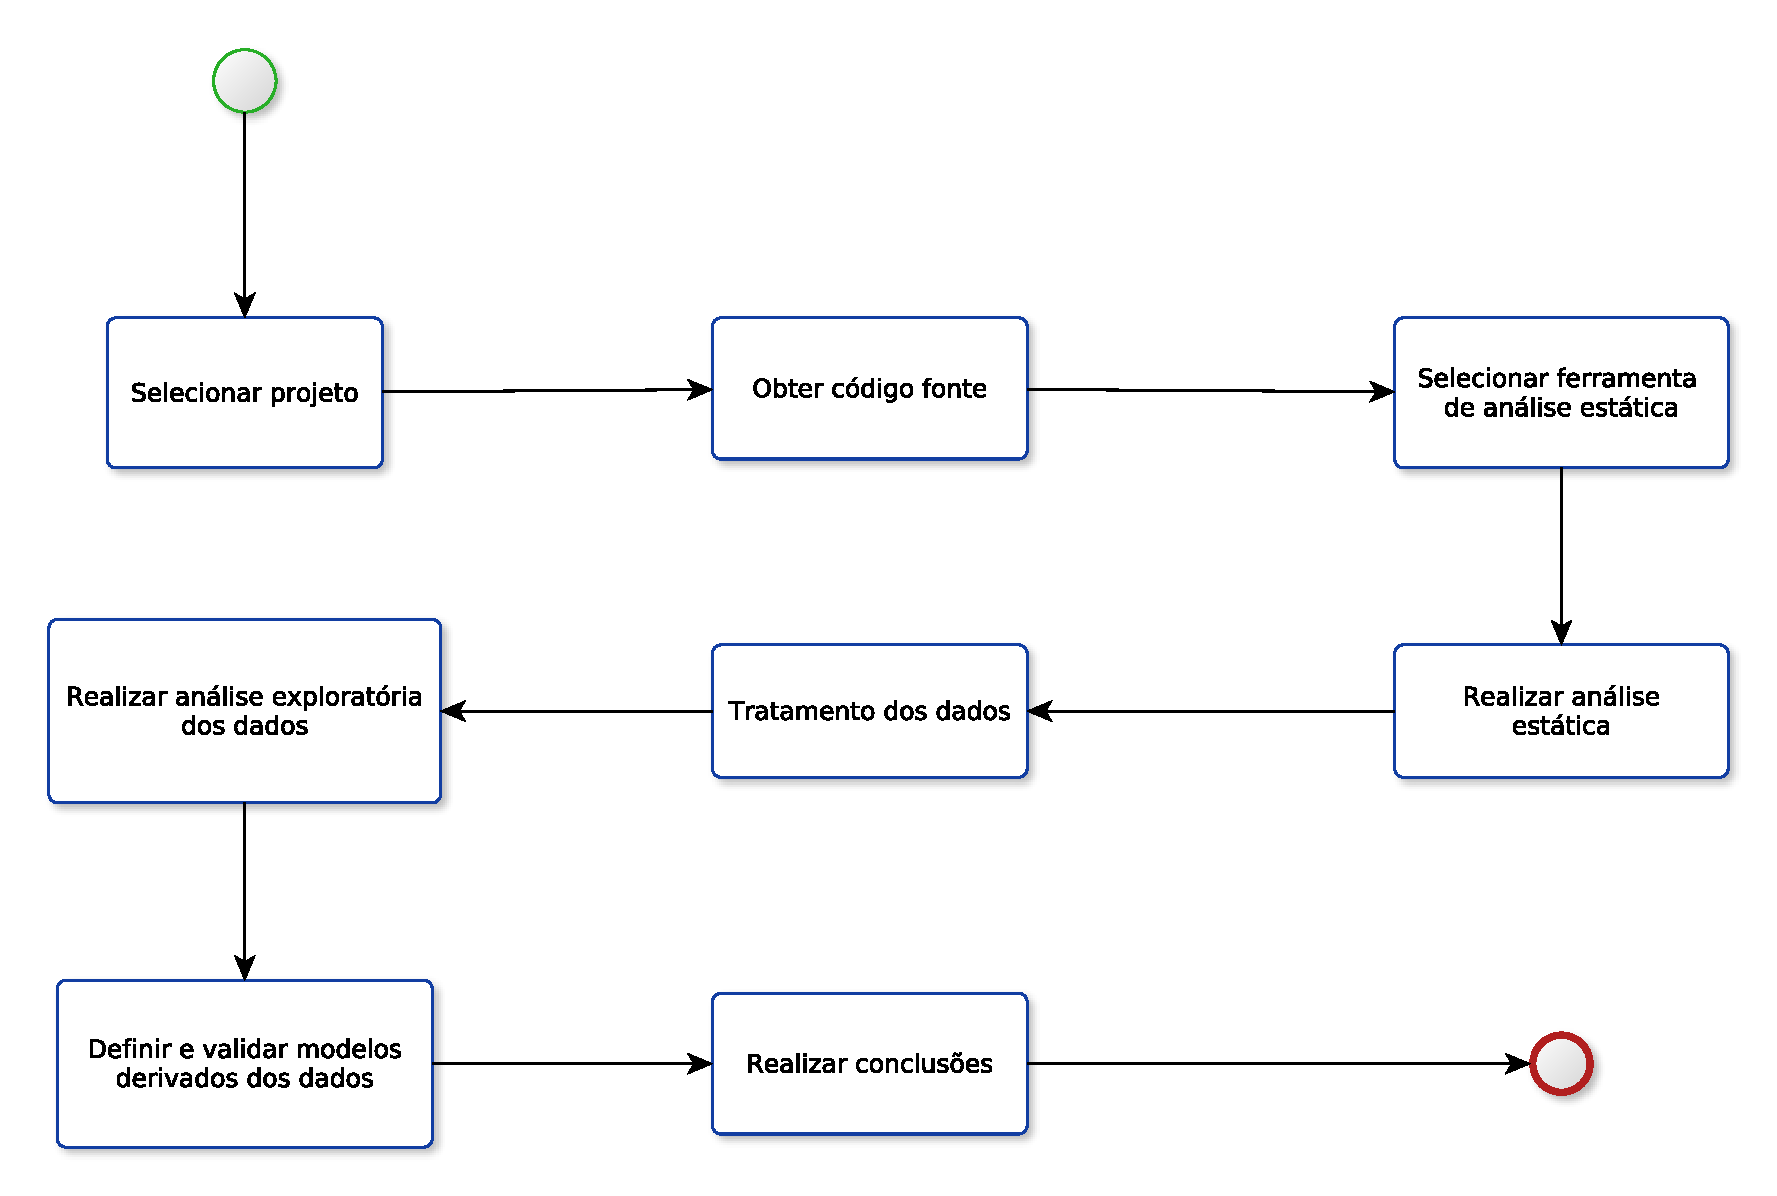
\includegraphics[width=0.9\textwidth]
      {figuras/metodologia_processo.eps}
  \caption{Processo contendo atividades executadas durante a pesquisa}
  \label{fig:processo}
\end{figure}

Detalhamento das atividades apresentadas na Figura \ref{fig:processo}:

\begin{enumerate}
  \item \textbf{Selecionar projeto}: Selecionar projeto de software livre
  representativo no contexto de segurança, para que possa ser feita a análise
  sobre o mesmo. O projeto deve ser um projeto já consolidado e com várias
  versões para que possa ser feita uma análise através do tempo.

  \item \textbf{Obter código fonte}: Obter código fonte das versões disponíveis
  do projeto selecionado, para que possa ser realizada a análise estática. A
  obtenção do código fonte deve ser feita de forma automatizada.

  \item \textbf{Selecionar ferramenta de análise estática}: Analisando os pontos
  fortes e fracos das ferramentas disponíveis, selecionar a ferramenta que
  melhor se adeque ao contexto em questão.

  \item \textbf{Realizar análise estática}: Realizar a análise estática sobre o
  código fonte obtido com a ferramenta selecionado de maneira automatizada.

  \item \textbf{Tratamento dos dados}: Ajustar o formato de saída da ferramenta
  utilizada para um arquivo CSV (\textit{Common Separated Values}) se a
  ferramenta não prover, além de tratar os dados descartando o que não for
  preciso e compondo os dados para gerar novos dados se necessário. Também deve
  ser feito de forma automatizada.

  \item \textbf{Realizar análise exploratória dos dados}: Utilizando uma
  ferramenta estatística, explorar os dados a fim de entender o comportamento do
  mesmo, para que facilite a dedução de um modelo próximo do real.

  \item \textbf{Definir e validar modelos derivados dos dados}: Encontrar
  modelos estatísticos (funções matemáticas) para monitoramento, acompanhamento e
  previsão das métricas de ameaças de vulnerabilidade de código fonte. Validar
  os modelos com dados cujo os quais não foram contruídos.

  \item \textbf{Realizar conclusões}: Comparar os modelos definidos e validados
  e indicar qual seria o melhor modelo para o monitoramento, acompanhamento e
  previsão das métricas em questão.
\end{enumerate}


\section{Testes das hipóteses}\label{metodologia:testeshipoteses}

Nesta sessão será descrito como foram feitos os testes das hipóteses levantadas
anteriormente. Para isso foram realizadas as atividades listadas na seção
\ref{metodologia:planejamentopesquisa}, figura \ref{fig:processo}.

O projeto selecionado para testar as hipóteses foi o \textit{Linux Kernel},
assim como o mesmo foi selecionado em \citeonline{cathedral_bazaar:1997} para se
estudar a engenharia de software. Devido o \textit{Linux Kernel} seguir um
modelo \textit{Bazaar} de desenvolvimento \cite{cathedral_bazaar:1997}, a
correção de \textit{bugs}, possíveis ameaças de vulnerabilidade, se dá de
maneira muito mais rápida, o que torna interessante a análise dessa nova classe
de métricas em um software bastante consolidado. Sendo esse o primeiro projeto a
explorar a rede de colaboração de software livre nos moldes atuais
\cite{cathedral_bazaar:1997}, tornando-se uma referência. Partiu-se do
\textit{Linux Kernel} para se estudar sobre práticas de desenvolvimento de
software e a própria engenharia de software, e agora será dado o primeiro passo
com relação a definição de um modelo estatístico que auxilie no monitoramento de
métricas de ameaças de vulnerabilidade de código fonte.

O código fonte do projeto \textit{Linux Kernel} foi obtido no espelho
(\textit{mirror}) do Github\footnote{\url{https://github.com/torvalds/linux}}
do repositório oficial Git do
projeto\footnote{\url{https://git.kernel.org/cgit/}}.  Fez-se uma cópia local
do repositório e foram utilizados alguns comandos \textit{bash} (via terminal)
para que a obtenção do código de todas as \textit{tags} disponíveis fosse feita
de uma única vez. Nesse repositório não havia as \textit{tags} de todas as
versões, pois o projeto passou a utilizar o Git\footnote{Ferramenta de controle
de versão descentralizado} apenas a partir da versão 2.6.11, entretanto, foi
possível obter o código de 391 \textit{tags} (da versão 2.6.11 até 3.9, contando
com todas as \textit{releases candidates} ou \textit{releases} intermediárias),
sendo considerado um número representativo e suficiente para a realização do
estudo.

A ferramenta de análise estática de código fonte selecionada para a realização
deste estudo foi o
\textit{Cppcheck}\footnote{\url{http://cppcheck.sourceforge.net/}}.  A parte
inicial da pesquisa se deu com a ferramenta \textit{Clang Static
Analyzer}\footnote{\url{http://clang-analyzer.llvm.org/}}(um submódulo do
compilador \textit{Clang}), esta ferramenta é bem completa e consegue capturar
bem as ameaças de vulnerabilidade de código fonte, entretanto, ela faz uma
análise inter-procedural do código, o que necessita da compilação do mesmo.
Infelizmente, o projeto \textit{Linux Kernel} ainda não suporta a sua total
compilação utilizando outro compilador a não ser o
GCC\footnote{\url{https://gcc.gnu.org/}}. Existe um projeto chamado
\textit{LLVMLinux
Project}\footnote{\url{http://llvm.linuxfoundation.org/index.php/Main_Page}} que
está tentando fazer com que o \textit{Linux Kernel} possa ser compilado com o
\textit{Clang}, mas esse trabalho ainda está em andamento. Logo, decidiu-se
abandonar o \textit{Clang Static Analyzer} e encontrar uma analisador estático
cujo qual não fosse necessária a compilação do código fonte, sendo esse o
\textit{Cppcheck}, que apesar de não realizar uma análise inter-procedural, ele
se propõe a não emitir uma grande quantidade de falsos positivos, chamada
ferramenta \textit{sound}.
